\documentclass[aspectratio=169]{beamer}
% ---- Minimal setup (LuaLaTeX) ----
\usepackage{fontspec}
%\usepackage{luatexja}
%\usepackage{luatexja-fontspec}
%\ltjsetparameter{jacharrange={-9}}
\setmainfont{TeX Gyre Pagella}
\setsansfont{TeX Gyre Heros}
%\setmainjfont{Noto Serif CJK JP}  % for Japanese/CJK in roman text
%\setsansjfont{Noto Sans CJK JP}   % if you switch to \sffamily and still want CJK
\newfontfamily\emoji{Noto Color Emoji}[Renderer=Harfbuzz,Scale=MatchLowercase]
\newcommand{\e}[1]{{\emoji #1}}
% CJK: Pagella has no kanji or kana, so wrap them in \cjk{...} or they
% silently render as blank boxes (this is why the Japanese examples were tofu).
\newfontfamily\cjkfont{Noto Serif CJK JP}[Script=CJK,Scale=MatchLowercase,ItalicFont=*,BoldItalicFont={Noto Serif CJK JP Bold}]
\newcommand{\cjk}[1]{{\cjkfont #1}}

% Dates come from web/weeks.toml via make_dates.py -- never type one.
% Generated by make_dates.py from web/weeks.toml -- do not edit.
% Change the timetable there, then run ./freeze.sh.
% Academic year: 2026

\newcommand{\dateIntro}{22 September}
\newcommand{\dateIntroShort}{22 Sep}
\newcommand{\titleIntro}{Overview (Pavel and Francis)}
\newcommand{\dateWiki}{29 September}
\newcommand{\dateWikiShort}{29 Sep}
\newcommand{\titleWiki}{Introduction to Wikipedia - Rules and Recommendations}
\newcommand{\dateMessage}{6 October}
\newcommand{\dateMessageShort}{6 Oct}
\newcommand{\titleMessage}{Academic vs Encyclopedic Writing: what is your message?}
\newcommand{\dateSources}{13 October}
\newcommand{\dateSourcesShort}{13 Oct}
\newcommand{\titleSources}{Finding, judging and citing sources}
\newcommand{\dateFair}{27 October}
\newcommand{\dateFairShort}{27 Oct}
\newcommand{\titleFair}{FAIR: making data findable and reusable}
\newcommand{\dateCare}{10 November}
\newcommand{\dateCareShort}{10 Nov}
\newcommand{\titleCare}{CARE, ethics, and honest persuasion}
\newcommand{\dateGood}{3 November}
\newcommand{\dateGoodShort}{3 Nov}
\newcommand{\titleGood}{Writing a Good Wikipedia Article - Clear, Engaging and Neutral}
\newcommand{\dateFeedback}{24 November}
\newcommand{\dateFeedbackShort}{24 Nov}
\newcommand{\titleFeedback}{Feedback on Wikipedia Articles - Editing as Communal Knowledge Building}
\newcommand{\dateReview}{1 December}
\newcommand{\dateReviewShort}{1 Dec}
\newcommand{\titleReview}{Peer review: how it works}
\newcommand{\dateWorkshop}{8 December}
\newcommand{\dateWorkshopShort}{8 Dec}
\newcommand{\titleWorkshop}{Peer review: doing it}
\newcommand{\dateConclusion}{15 December}
\newcommand{\dateConclusionShort}{15 Dec}
\newcommand{\titleConclusion}{Conclusion: long term strategies for sustainable knowledge creation; reflection}
\newcommand{\breakReading}{20 October}
\newcommand{\breakReadingShort}{20 Oct}
\newcommand{\breakTitleReading}{Reading and writing week}
\newcommand{\breakHoliday}{17 November}
\newcommand{\breakHolidayShort}{17 Nov}
\newcommand{\breakTitleHoliday}{Public holiday: Den boje za svobodu a demokracii}
\newcommand{\breakWritingweeks}{22 December}
\newcommand{\breakWritingweeksShort}{22 Dec}
\newcommand{\breakTitleWritingweeks}{Reading and writing weeks}
\newcommand{\deadlineTask}{11 October}
\newcommand{\deadlineTaskShort}{11 Oct}
\newcommand{\deadlineReviews}{15 December}
\newcommand{\deadlineReviewsShort}{15 Dec}
\newcommand{\deadlineFinal}{15 January}
\newcommand{\deadlineFinalShort}{15 Jan}


\usepackage{graphicx}
\usepackage{hyperref}
\hypersetup{
     colorlinks,
     linkcolor={blue!50!black},
     citecolor={red!50!black},
     urlcolor={blue!80!black}
   }
\usepackage{booktabs}
\usepackage{microtype}

\newcommand{\txx}[1]{\textbf{\textcolor{blue}{#1}}}

% --- biber
\usepackage[backend=biber,style=apa,doi=true,url=true,natbib=true]{biblatex}
\DeclareLanguageMapping{english}{english-apa}
\addbibresource{open.bib}

% ---- Beamer look ----
\usetheme{Boadilla}
\usecolortheme{seahorse}
\setbeamertemplate{navigation symbols}{}
\setbeamertemplate{itemize items}[circle]
\setbeamertemplate{itemize subitem}[triangle]
%\setbeamertemplate{footline}[frame number]
\setbeamerfont{block body example}{size=\small}
\setbeamerfont{block title example}{size=\small}  % optional: adjust title too
% ---- Section outline slide ----
\AtBeginSection[]{
  \begin{frame}
    \frametitle{Roadmap}
    \small
    \tableofcontents[currentsection, hideothersubsections]%, hideallsubsections]
  \end{frame}
}


% ---- other packages
\usepackage{tikz}

% ---- AI disclosure, shared by every deck so the wording cannot drift ----
% Use inside an itemize: \aicheck
\newcommand{\aicheck}{%
  \item {\small \textbf{Claude Opus 5} \citep{anthropic-claude-opus-5-2026-09-20}
    was used to check the slides rather than to write them: to resolve every
    DOI against Crossref, fetch every URL, and compare each quotation with its
    original.  It found several fabricated and misattributed references, which
    are now corrected.  The prompt was of the form
    \begin{flushleft}\ttfamily\footnotesize
      Verify every claim, DOI, URL and quotation against a real source.  Where
      you cannot verify something, say so rather than guessing --- never
      invent a reference. \\
    \end{flushleft}
    Each correction names the source it was checked against.  Responsibility
    for what remains is mine.}%
}


% ---- Title metadata ----
\title[Feedback]{Open Knowledge for a Sustainable Future:\\ Research, Ethics, and Wikipedia}
\subtitle{Week 7  — Feedback on Academic Articles - Peer review and revision for publication}
\author[Bond \& Bednařík]{Francis Bond (\textbf{Academic}) \and Pavel Bednařík (Wiki)}
\institute[UPOL \& Wikimedia]{Palacký University Olomouc \quad | \quad Wikimedia ČR}
\date{2025-12-06}

\begin{document}

% =====================================================================
\begin{frame}
  \titlepage
\end{frame}

% ======================================
% Feedback & Writing: The foundation for peer review
% ======================================
\section{Feedback and Revision}

\begin{frame}{Writing is a process — feedback is essential}
\begin{itemize}
  \item First drafts are rarely clear, complete, or well-argued
  \item Feedback (from peers, tutors, self-reflection) helps identify:
    \begin{itemize}
    \item unclear claims
    \item logical gaps
    \item missing evidence
    \item stylistic issues
    \end{itemize}
  \item Improving writing increases clarity, persuasiveness, and ethical responsibility — especially important when dealing with data, culture, or community topics
\end{itemize}
\end{frame}

\begin{frame}{What feedback gives to the writer}
\begin{itemize}
  \item Another reader's perspective — reveals assumptions or blind spots
  \item Fresh eyes on structure, coherence, and flow: does argument build logically?
  \item Opportunity to strengthen evidence and address counter-arguments
  \item Chance to improve style, tone, and accessibility depending on audience
\end{itemize}
\end{frame}

\begin{frame}{Feedback benefits the critical reader too}
\begin{itemize}
  \item Readers become more critical and informed — able to assess evidence, question assumptions, and spot weak arguments
  \item Improves collective standards: better writing leads to better discourse
  \item Feeds back into research culture: clarity and transparency help others replicate, critique, or build further work
\end{itemize}
\end{frame}

\begin{frame}{Feedback is ethical, not just cosmetic}
\begin{itemize}
  \item Writing about people, cultures, data — carries responsibility. Feedback helps catch problematic framing, bias, or unintended harm
  \item Encourages accountability: facts must be checked, sources verified, sensitive topics handled with care
  \item Discipline-wide benefit: careful writing builds trust, respect, and legitimacy for scholarship
\end{itemize}
\end{frame}


% =========================
% Week 7 — Peer Review, Trust, and Metrics
% =========================
\section{Peer Review, Trust, and Metrics}

% --- WHAT PEER REVIEW IS
\begin{frame}{What peer review is}
\begin{itemize}
  \item Peer review is the process by which experts evaluate a manuscript before publication
  \item Its aims are to:
    \begin{itemize}
      \item Check the \textbf{soundness} of methods and argument
      \item Improve clarity, structure, and contribution
      \item Build \textbf{trust} in published research
    \end{itemize}
  \item Reviewers act as gatekeepers and mentors — ideally improving the quality of science and scholarship
\end{itemize}
\textit{Peer review is not about perfection; it is about accountability and conversation.}
\end{frame}

% --- TYPES OF PEER REVIEW
\begin{frame}{Types of peer review}
\begin{itemize}
  \item There are several models of peer review, each balancing \textbf{transparency, fairness, and accountability} in different ways
\end{itemize}

\begin{description}
  \item[Single-blind:] Reviewers know the author's identity, but authors do not know the reviewers
    \begin{itemize}
      \item Common in science and social science
      \item Advantage: reviewers can assess expertise and potential conflicts
      \item Risk: unconscious bias (e.g., by gender, affiliation, language, or region)
    \end{itemize}

  \item[Double-blind:] Neither authors nor reviewers know each other's identity
    \begin{itemize}
      \item Aims to reduce bias and level the playing field
      \item Often used in humanities and linguistics conferences
      \item Risk: anonymity may limit accountability; reviewers can sometimes guess authors
    \end{itemize}

  \item[Open review:] Both sides know identities, and sometimes reviews are published
    \begin{itemize}
      \item Promotes transparency and recognition of reviewing labour
      \item Encourages constructive tone, but may discourage strong criticism
      \item Used in some open-science and data journals
    \end{itemize}
\end{description}

% \medskip
% \textit{Each model reflects what a community values most — fairness, openness, or candour.}
 \end{frame}



% --- STRENGTHS AND WEAKNESSES
\begin{frame}{Peer review: strengths and weaknesses}
\begin{columns}[T]
\column{0.48\textwidth}
\textbf{Strengths}
\begin{itemize}
  \item Enhances rigour and precision
  \item Provides expert feedback before publication
  \item Establishes a shared standard of credibility
  \item Encourages dialogue within a discipline
\end{itemize}

\column{0.48\textwidth}
\textbf{Weaknesses}
\begin{itemize}
  \item Can be slow, inconsistent, or biased
  \item Overburdens a small reviewer pool
  \item Replication and transparency not always checked
  \item Negative or null results often unpublished ("file-drawer" effect)
\end{itemize}
\end{columns}
\medskip
\textit{Peer review is essential but imperfect — a social process as much as a scientific one.}
\end{frame}

% --- EMERGING ALTERNATIVES (with hyperlinks)
\begin{frame}{Evolving models of peer review}
\begin{itemize}

  \item \textbf{Post-publication review:}
    \begin{itemize}
      \item Articles or datasets are published first, then openly discussed
      \item Examples: 
        \href{https://f1000research.com/}{F1000Research}, 
        \href{https://pubpeer.com/}{PubPeer}
    \end{itemize}

  \item \textbf{Community review:}
    \begin{itemize}
      \item Large-scale collaborative commenting before publication  
            (e.g., open preprints, \href{https://github.com/}{GitHub issues}, \href{https://langsci-press.org/openReview/intro}{Open Review at LangSci Press})
      \item Builds transparency and collective expertise
    \end{itemize}

  \item \textbf{Preprint feedback:}
    \begin{itemize}
      \item Early sharing (e.g., \href{https://arxiv.org/}{arXiv}, 
            \href{https://ling.auf.net/lingbuzz}{LingBuzz}) invites informal peer feedback before formal submission
      \item Speeds dissemination and reduces "scoop" anxiety
    \end{itemize}

  \item These models shift peer review from an evaluation to a 
       conversation
\end{itemize}

\end{frame}


% --- RESPONSIBILITIES AND ETHICS OF REVIEWERS
\begin{frame}{Ethical responsibilities of peer reviewers}
\begin{itemize}
  \item Reviewers are entrusted with \textbf{privileged access} to unpublished work
  \item Ethical responsibilities include:
    \begin{itemize}
      \item \textbf{Confidentiality}: do not share, quote, or use ideas from the manuscript
      \item \textbf{Impartiality}: declare conflicts of interest; avoid personal or institutional bias
      \item \textbf{Constructive criticism}: focus on improving the work, not attacking the author
      \item \textbf{Timeliness}: return reviews promptly; long delays can harm authors' careers
      \item \textbf{Accuracy}: evaluate methods, evidence, logic, and citations fairly
      \item \textbf{Respect}: use professional tone; assume good intent; avoid dismissive language
    \end{itemize}
  \item As \citet{rockwell2005prethics} emphasises, access to unpublished research creates a
        \textbf{power imbalance}: reviewers must not exploit this advantage
\end{itemize}
\medskip
\textit{A good reviewer protects confidentiality, improves clarity, and strengthens trust in scholarship.}
\end{frame}


% ================================
% Feedback in Industry: Giving Notes
% ================================
\subsection{Feedback Beyond Academia}

\begin{frame}{Feedback in industry: the practice of "giving notes"}
\begin{itemize}
  \item In many industries (film, publishing, games, advertising), feedback is formalised as \textbf{"notes"} \citep{catmull2014creativityinc}
  \item Notes come from editors, producers, managers, clients — often in a hierarchical chain
  \item The goal is similar to academic review:
    \begin{itemize}
      \item improve clarity, impact, and quality
      \item ensure the work meets its purpose and audience
    \end{itemize}
  \item But constraints differ:
    \begin{itemize}
      \item strict deadlines, budgets, brand guidelines, legal concerns
      \item competing visions between writer/creator, editor, and client
    \end{itemize}
\end{itemize}

\medskip
\small Video: \href{https://www.youtube.com/watch?v=I1Mr3oKR7oM}{Ed Catmull on the Pixar Braintrust} (Stanford, 8 min) %% SHOW IN CLASS?
\end{frame}

\begin{frame}{How industry notes differ from academic peer review}
\begin{itemize}
  \item \textbf{Hierarchical:} notes often come from someone with authority over the project (editor, producer, manager)
  \item \textbf{Goal-driven:} feedback must serve the needs of the project, brand, or product — not the advancement of knowledge
  \item \textbf{Collaborative but constrained:} creators negotiate changes, but ultimate decisions may be external
  \item \textbf{Iterative cycles:} multiple rounds of notes → revisions → more notes → final approval
  \item \textbf{Success = alignment} with project goals, not independent scholarly rigour
\end{itemize}

\end{frame}

\begin{frame}{Best practices from industry feedback culture}
\begin{itemize}
  \item \textbf{Clarity first:} Notes should define the problem before proposing solutions (Pixar rule)
  \item \textbf{Respect creative intent:} Improve the work without imposing a personal style
  \item \textbf{Prioritise high-impact changes:} Not all notes can be addressed; choose the ones that serve the project
  \item \textbf{Negotiate professionally:} Creators can ask for clarification and push back when necessary
  \item \textbf{Shared responsibility:} Good notes identify issues; creators choose how to solve them
\end{itemize}

\end{frame}

\begin{frame}{What students can learn from industry feedback}
\begin{itemize}
  \item You will encounter feedback in many forms: editorial, managerial, client-oriented, or technical
  \item Key transferable skills:
    \begin{itemize}
      \item receiving feedback without defensiveness
      \item interpreting conflicting goals
      \item deciding which suggestions to adopt, adapt, or reject
      \item communicating clearly about revisions
    \end{itemize}
  \item Ethical themes remain:
    \begin{itemize}
      \item respect, clarity, collaboration, responsibility
    \end{itemize}
\end{itemize}
\textit{Good feedback — academic or industrial — improves the work and strengthens the team.}
\end{frame}


% ================================
% Feedback beyond academia
% ================================

\begin{frame}{Feedback cultures beyond academic peer review}
\begin{itemize}
  \item \textbf{Journalism:} Editors and fact-checkers verify claims against primary sources before publication — different from academic review, which often assumes sources are cited correctly
  \item \textbf{Wikipedia:} Articles pass through multiple stages of community review; good/featured article criteria require verifiability and neutral point of view
  \item \textbf{Code review:} In software development, peers review code for bugs, style, and maintainability — feedback is typically public and tied to version control (e.g., GitHub pull requests)
  \end{itemize}
\medskip
  \textit{Feedback aims to improve quality through structured critique before the results are made public}
\end{frame}


\subsection{Reviewing at the Association for Computational Linguistics}
% ======================================
% ACL CONTEXT & WHY WE STUDY PEER REVIEW
% ======================================

\begin{frame}{Peer review in Computational Linguistics}
\begin{itemize}
  \item Peer review is so central to scholarship that whole communities invest in improving it
  \item The Association for Computational Linguistics (ACL) publishes:
    \begin{itemize}
      \item reviewer training guides \citep{acl2023reviewbasics}
      \item best-practice recommendations  \citep{aclarrguidelines}
      \item annual reports analysing what works and what fails \citep{aclcopr2023}
    \end{itemize}
  \item These offer a model for responsible, constructive, ethical reviewing
  \item ACL 2025 followed the following structure:
    \begin{itemize}
    \item  8,300 submissions
    \item  1,700 accepted as full,  1,392 as findings
      % (/ 17 83.0) 0.20481927710843373
    \item  169 Senior Area Chairs, 1,937 Area Chairs, 11,720 reviewers!
    \item Each paper reviewed by three reviewers, the authors respond, the reviewers update their reviews,  the area chairs suggest which papers are accepted, the senior area chairs make the final decisions, \ldots
    \end{itemize}
\end{itemize}
\end{frame}

% ======================================
% BASICS: QUALIFICATION & CONFLICTS
% ======================================

\begin{frame}{Accept reviews only when appropriate (ACL guidelines)}
\begin{itemize}
  \item Before agreeing to review, check:
    \begin{itemize}
      \item \textbf{Expertise}: Can you fairly assess the methods and claims?
      \item \textbf{Conflicts of interest}: shared institution, collaborators, competitors
      \item \textbf{Capacity}: Do you actually have time to read carefully?
    \end{itemize}
  \item Accepting when you are unqualified or overloaded leads to unfair or rushed reviews
  \item Slightly undermined by the fact that if you submit a paper you must agree to review at least 5 others, \ldots
      \begin{itemize}
    \item ACL has a 15-20\% acceptance rate, so for one paper accepted 4 are rejected. 

    \end{itemize}
\end{itemize}

\end{frame}

% ======================================
% STRATEGIC READING
% ======================================

\begin{frame}{Read carefully and generously (ACL guidelines)}
\begin{itemize}
  \item First read: understand the research question and contribution
  \item Second read: evaluate evidence, structure, and clarity
  \item Look for what the author is \emph{trying} to do
  \item Avoid snap judgments based on style, formatting, or first impressions
\end{itemize}

\end{frame}

% ======================================
% CONSTRUCTIVE, ACTIONABLE FEEDBACK
% ======================================

\begin{frame}{Write constructive, actionable feedback (ACL guidelines)}
\begin{itemize}
  \item Every review should include both:
    \begin{itemize}
      \item \textbf{Strengths} — what works well
      \item \textbf{Weaknesses} — what needs improvement
    \end{itemize}
  \item Make criticisms specific:
    \begin{itemize}
      \item point to a sentence or section
      \item explain why it is unclear
      \item suggest how to fix it
    \end{itemize}
  \item Vague comments (\textit{paper is confusing}) are unhelpful
\end{itemize}

\end{frame}

% ======================================
% CHECK ETHICS, REPRODUCIBILITY, FAIRNESS
% ======================================

\begin{frame}{Check evidence, ethics, and reproducibility (ACL guidelines)}
\begin{itemize}
  \item A reviewer is responsible for more than novelty
  \item Consider:
    \begin{itemize}
      \item Are claims supported by evidence?
      \item Are methods and data described clearly?
      \item Are ethical implications acknowledged?
      \item Can results be verified or reproduced?
    \end{itemize}
  \item Responsible peer review strengthens the entire field
\end{itemize}

\end{frame}

% ======================================
% PROFESSIONALISM & RESPECT
% ======================================

\begin{frame}{Professionalism and respect (ACL guidelines)}
\begin{itemize}
  \item Use a constructive and collegial tone
  \item Avoid dismissive language:
    \begin{itemize}
      \item "This is trivial"
      \item "obviously wrong"
      \item "the authors don't understand"
    \end{itemize}
  \item Remember: reviewers and authors are colleagues
  \item Treat the paper the way you would want yours to be treated
\end{itemize}

\end{frame}

% ======================================
% POWER & RESPONSIBILITY
% ======================================

\begin{frame}{Reviewer power and responsibility (ACL COPR)}
\begin{itemize}
  \item Reviewers gain \textbf{access to unpublished work} before the community
  \item This creates responsibility:
    \begin{itemize}
      \item Never use unpublished ideas in your own work
      \item Never delay a review to gain priority
      \item Never punish papers that challenge your favourite theory
    \end{itemize}
  \item Peer review is a trust-based system; unethical reviewing harms entire fields
\end{itemize}

\end{frame}

% ======================================
% WHAT THIS MEANS FOR STUDENTS
% ======================================

\begin{frame}{What this means for you (student reviewers)}
\begin{itemize}
  \item The same principles apply in the classroom:
    \begin{itemize}
      \item read generously
      \item comment specifically
      \item focus on clarity, evidence, and logic
      \item be respectful and supportive
    \end{itemize}
  \item Practising good peer review improves your own writing:
    \begin{itemize}
      \item you learn what makes an argument work
      \item you see how readers interpret drafts
      \item you build editorial judgment
    \end{itemize}
\end{itemize}
\medskip
\small  Based on ACL reviewer training materials \citep{acl2023reviewbasics, aclarrguidelines, aclcopr2023}.
\end{frame}

% ======================================
% SUMMARY SLIDE
% ======================================

\begin{frame}{ACL-inspired peer review checklist}
\begin{itemize}
  \item Am I qualified and conflict-free?
  \item Have I read the paper carefully (twice)?
  \item Did I identify strengths and weaknesses?
  \item Are my comments specific and actionable?
  \item Did I evaluate ethics, evidence, and reproducibility?
  \item Is my tone respectful and professional?
  \item Have I upheld confidentiality and integrity?
\end{itemize}

\end{frame}


\section{Problems: Bias \& Inequality, (un)Reproducibility}
\subsection{Punktoza}
\begin{frame}{Publish or Perish}

  \begin{itemize}
  \item Academics are under pressure to publish
  \item This is a major part of how they are evaluated
  \item This should lead to more, higher quality publications
  \item But can lead to many more, lower  quality publications
    \begin{itemize}
    \item Or even fraud!
    \end{itemize}
  \item And means we have to review more and more publications
  \end{itemize}
  
\end{frame}

% --- METRICS: WHY THEY WERE INTRODUCED
\begin{frame}{Metrics: why they were introduced}
\begin{itemize}

  \item Growing research ecosystems needed \textbf{standardised indicators} to compare:
    \begin{itemize}
      \item journals (Impact Factor)
      \item researchers (h-index)
      \item institutions (citation counts, productivity)
    \end{itemize}

  \item \textbf{Impact Factor (IF):} average number of citations to articles in a journal over a two-year period
  \begin{itemize}
    \item Designed to help libraries choose journals and to signal visibility
  \end{itemize}

  \item \textbf{h-index:} a researcher has index $h$ if they have $h$ papers each cited at least $h$ times
  \begin{itemize}
    \item Intended to combine productivity + influence in a single number
  \end{itemize}

  \item Metrics aimed to make evaluation \textbf{transparent, comparable, and data-driven}
  \item They were introduced to help — not to replace — expert judgment

\end{itemize}
\end{frame}


% --- METRICS: PROBLEMS, GOODHART, PUNKTOZA
\begin{frame}{Metrics: when measures become targets}
\begin{itemize}

  \item When hiring, promotion, or funding is tied to metrics:
  \begin{itemize}
    \item Researchers optimise for what is counted, not what is meaningful
    \item Citation counts become currency; novelty outranks replication or rigour
  \end{itemize}

  \item \textbf{Goodhart's Law:}
  \begin{quote}
    When a measure becomes a target, it ceases to be a good measure.
  \end{quote}
  \vspace*{-2.5ex}
  \begin{itemize}
    \item IF and h-index lose validity once people actively game them
  \end{itemize}

  \item \textbf{Punktoza ("points fever"):} publishing strategically to accumulate evaluation points rather than to advance knowledge \citep{kulczycki2017punktoza,kulczycki2017assessing}
  \begin{itemize}
    \item Encourages salami-slicing, low-risk incremental work, quantity over substance
    \item A systemic response to metric-driven national evaluation frameworks
  \end{itemize}

  \item Metrics intended to guide evaluation end up \textbf{shaping behaviour}, sometimes harming scholarship

\end{itemize}

\textit{Quantifying trust can erode it when numbers replace judgment.}
\end{frame}


\begin{frame}{Goodhart's Law  \href{https://xkcd.com/2899/}{xkcd 2899}}
  \begin{center}
    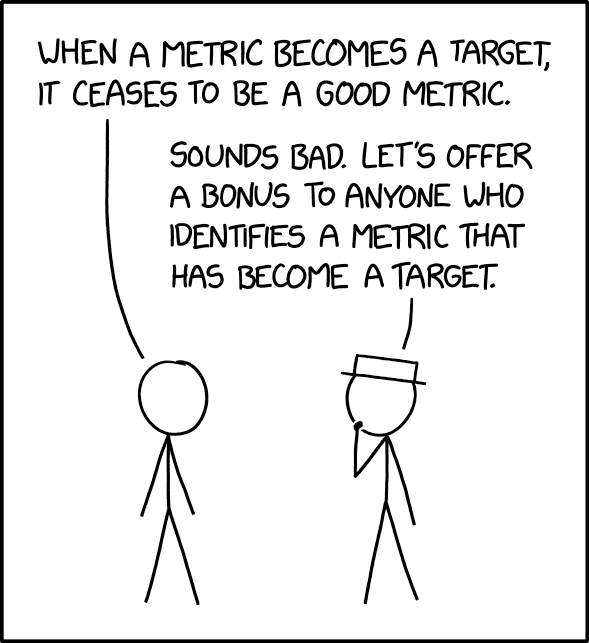
\includegraphics[width=0.45\textwidth]{img/goodharts_law_2x.png}
  \end{center}
\end{frame}

% ===================================
% Bias and Inequality in Peer Review
% ===================================

\subsection{Bias and Inequality in Peer Review}
\begin{frame}{Peer review is not neutral — known biases}
\begin{itemize}
  \item Peer review should be meritocratic — but social biases can shape outcomes
  \item Empirical studies document systematic bias based on gender, institutional prestige, and affiliation
  \item This can reproduce inequalities in academic visibility and access
\end{itemize}
\end{frame}

\begin{frame}{Gender bias and underrepresentation}
\begin{itemize}
  \item A large study of 1.7 million authors and 740,000 referees found that manuscripts by women were not universally penalized — yet women remain under-represented among peer reviewers and editors \citep{helmer2017genderbias}
  \item Another review finds that women are less likely to appear as first/last authors, especially in high–impact journals, and are underrepresented as reviewers/editors
    \citep{murray2020genderpeerreview}
  \item In grant-review contexts, women have also been shown to receive lower scores despite similar qualifications
    \citep{wenneras1997nepotism}
  \end{itemize}
\end{frame}

\begin{frame}{Institutional – affiliation and prestige bias}
\begin{itemize}
\item Recent evidence shows "affiliation bias": papers from prestigious or well-known institutions are more likely to get favourable review or acceptance
  \citep{tomkins2017dblblind}
  \item This can disadvantage authors from lesser-known institutions, even when the manuscript quality is comparable
  \item Result: citation networks and publication records amplify institutional inequality — making "the rich institutions" richer
\end{itemize}
\end{frame}

\begin{frame}{Why these biases happen — and what can we do?}
  \begin{itemize}
  \item Why these biases happen
    \begin{itemize}
    \item Reviewers (and editors) may rely on stereotypes, familiarity, or "status cues" (institution name, authors' reputation) rather than content
    \item Reviewing is human work; unconscious bias — on gender, prestige, nationality, career stage — is common
    \item Peer-review bias is not just about individual reviewers, but structural patterns: who gets invited to review, whose papers get visibility, who gets accepted
    \end{itemize}
  \item What this means for us
    \begin{itemize}
    \item As reviewers: stay alert to bias. Evaluate based on content, not identity or institution
    \item As authors: be aware that results and visibility may be influenced by social factors beyond quality
    \item As a community: encourage diversity in reviewers/editors, anonymised review where possible, transparency in editorial decisions
    \item Use blind review where possible
    \end{itemize}
  \end{itemize}
\end{frame}


% ===================================
% The Reproducibility Crisis & Why It Matters
% ===================================
\subsection{The Reproducibility Crisis} 
\begin{frame}{What is reproducibility / replicability?}
\begin{itemize}
  \item \textbf{Reproducibility:} re-analyse the same data/code to get the same result
  \item \textbf{Replicability:} collect new data under same conditions and test whether the effect holds
  \item Both are fundamental for reliable knowledge — without them, published findings remain provisional \citep{goodman2016reproducibility}
\end{itemize}
\end{frame}

\begin{frame}{What the crisis looks like — some sobering numbers}
\begin{itemize}
\item In a 2015 project replicating 100 psychology studies, only ~36\% of results were successfully replicated; effect sizes dropped by about 50\% \citep{open2015reproducibility}
  
  \item A 2016 survey in biomedical research found over 70\% of researchers had tried and failed to reproduce another scientist's results — and 52\% judged that there is a significant crisis \citep{baker2016crisis}
  \item Fields like oncology (e.g.\ cancer-biology) show particularly low reproducibility: external audits of many "landmark" papers found < 1/3 of results reliably reproduced
   \citep{errington2021cancer}
\end{itemize}
\begin{block}{Why this matters}
If published findings routinely fail replication, the scientific literature becomes unreliable — which undermines trust, wastes resources, and misleads follow-up research.
\end{block}

\medskip
\small Video: \href{https://www.youtube.com/watch?v=42QuXLucH3Q}{Veritasium: "Is Most Published Research Wrong?"} (12 min) %% SHOW IN CLASS?
\end{frame}

\begin{frame}{Causes: why reproducibility fails}
\begin{itemize}
\item Low statistical power (too few subjects/samples) — leads to unstable, non-robust effects
   \citep{ioannidis2005false}
  \item Publication bias \& questionable research practices (QRPs): only positive or novel results tend to get published; null results stay hidden
  \item Poor documentation, missing code/data, hidden methods — even honest researchers make replication hard when they do not share full materials
  \item Time \& incentive structures: scientists rewarded for novelty, impact, and speed — not for replication or careful method sharing
\end{itemize}
\end{frame}

\begin{frame}{How FAIR + CARE + Good Writing helps fix reproducibility}
\begin{itemize}
  \item Proper metadata, shared code/data, and clear methods (FAIR) make re-analysis possible
  \item Ethical responsibility (CARE) encourages transparent, honest reporting — including limitations, context, and reproducibility risks
  \item Careful writing and documentation help readers understand exactly how a study was done
  \item Together — transparent data practices, open sharing + honest reporting 
    \item[=] more reliable science
\end{itemize}
\end{frame}

% --- CITATION AS TRUST
\begin{frame}{Citation as trust}
\begin{itemize}
  \item A citation is a \textbf{link of trust}: it says ``I have read and found this work reliable enough to build upon''
  \item Over time, citations form \textbf{networks of credibility} — maps of intellectual influence
  \item Not all citations are equal:
    \begin{itemize}
      \item Some endorse, others critique or merely mention
      \item "Citation cascades" can perpetuate unverified claims
    \end{itemize}
  \item Responsible citation means reading, understanding, and acknowledging context — not just counting links
\end{itemize}
\textit{Citation is conversation: each reference extends a thread of shared trust.}
\end{frame}

\begin{frame}{Citogenesis \href{https://xkcd.com/978/}{xkcd 978}}
  \begin{center}
    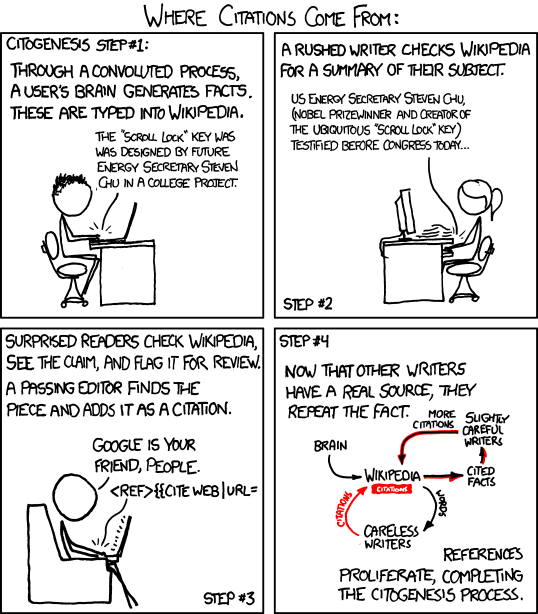
\includegraphics[width=0.4\textwidth]{img/citogenesis.png}
  \end{center}
\end{frame}

% ================================
% AI and Peer Review
% ================================
\subsection{AI and Peer Review}

\begin{frame}{AI in peer review: emerging concerns}
\begin{itemize}
  \item Large language models (LLMs) like ChatGPT are increasingly used in academic writing — and in peer review
  \item A 2024 study estimated that 6.5–17\% of peer reviews at major AI conferences may have been substantially written or modified by LLMs \citep{liang2024aireviews}
  \item Telltale signs: unusual adjectives ("commendable", "meticulous", "intricate") spiked 10–35× in frequency
  \item Major publishers (Springer Nature, Taylor \& Francis, Sage) now prohibit or restrict AI use in peer review
\end{itemize}
\end{frame}

\begin{frame}{Why AI-generated reviews are problematic}
\begin{itemize}
  \item \textbf{Confidentiality breach}: uploading a manuscript to an LLM shares it with a third party
  \item \textbf{Accountability}: reviewers are responsible for accuracy and judgment — LLMs cannot be held accountable
  \item \textbf{Bias and hallucination}: LLMs can perpetuate biases and produce plausible-sounding but incorrect critiques
  \item \textbf{Superficiality}: AI-generated reviews tend to be generic and miss domain-specific issues
  \item \textbf{Trust erosion}: if reviews are automated, peer review loses its meaning as expert evaluation
\end{itemize}
\medskip
\textit{Peer review depends on human expertise, judgment, and responsibility — qualities LLMs cannot replicate.}
\end{frame}

\begin{frame}{Current guidance on AI in peer review}
\begin{itemize}
  \item Most journals and conferences now require:
    \begin{itemize}
      \item Disclosure of any AI assistance in writing or reviewing
      \item Human accountability for all submitted content
      \item No uploading of confidential manuscripts to AI tools
    \end{itemize}
  \item Acceptable uses (with disclosure):
    \begin{itemize}
      \item Grammar and spell-checking
      \item Improving clarity of your own writing
    \end{itemize}
  \item Unacceptable uses:
    \begin{itemize}
      \item Generating review text
      \item Summarising or analysing manuscripts you are reviewing
      \item Submitting AI-generated content as your own expert judgment
    \end{itemize}
\end{itemize}
\end{frame}

\section{Peer Review \& Revision in Practice}

\begin{frame}{From theory to practice}
\begin{itemize}
  \item Peer review, reproducibility, and citation ethics all serve one purpose: maintaining credibility
  \item Today we practise this on a smaller scale:
    \begin{itemize}
      \item Read your partner's paper carefully
      \item Give specific, constructive, respectful feedback
      \item Remember: your review contributes to their improvement — and your own understanding of good writing
    \end{itemize}
\end{itemize}
\end{frame}


% --- WHY REVISION MATTERS (AGAIN)
\begin{frame}{Why revision matters (again)}
\begin{itemize}
  \item Good writing is \emph{rewriting}: clarity, structure, and claims improve with feedback
  \item Revision is not cosmetic editing; it is \textbf{rethinking} your argument and evidence
  \item Peer review helps you see what your reader actually understands
  \item Goal today: find \textbf{actionable changes} you can complete before final submission
\end{itemize}
\end{frame}

% --- WHAT PEER REVIEW IS (AND ISN'T)
\begin{frame}{What peer review is (and isn't)}
\begin{itemize}
  \item A reader's report on \textbf{clarity, evidence, logic, and structure}
  \item Specific, constructive, and respectful; focused on \textbf{the writing}, not the writer
  \item Not copyediting every comma; not "gotcha"
  \item[$\Rightarrow$] Prioritise the few changes with the biggest impact
\end{itemize}
\end{frame}

% --- HOW TO GIVE USEFUL FEEDBACK
\begin{frame}{How to give useful feedback}
\begin{itemize}
  \item Be \textbf{specific}: point to a sentence/paragraph and say what is unclear and why
  \item Be \textbf{diagnostic}: name the issue (claim lacks evidence; paragraph lacks topic sentence)
  \item Be \textbf{actionable}: propose a next step (add a source; move paragraph; define a term)
  \item Balance: 1–2 strengths + 1–2 high-value improvements
\end{itemize}
\end{frame}

% --- RESPONDING TO REVIEWS
\begin{frame}{How to respond to reviews}
\begin{itemize}
  \item \textbf{Read carefully}: understand what the reviewer is actually asking — not what you fear they mean
  \item \textbf{Respond to everything}: address each comment, even if briefly ("We have revised X as suggested" or "We respectfully disagree because Y")
  \item \textbf{Be specific in your response}: quote the comment, then explain exactly what you changed (with page/line numbers)
  \item \textbf{Don't be defensive}: assume good intent; reviewers are trying to improve your work
  \item \textbf{Push back professionally}: if you disagree, explain why with evidence — editors respect reasoned disagreement
  \item \textbf{Thank your reviewers}: they volunteered their time
\end{itemize}
\end{frame}

% --- REVIEWER DECODER
\begin{frame}{Reviewer comment decoder}
\small
\begin{tabular}{p{0.45\textwidth}p{0.45\textwidth}}
\textbf{What reviewers write} & \textbf{What they often mean} \\
\hline
"The motivation is unclear" & Your introduction doesn't explain why anyone should care \\
"This needs more context" & You assumed background knowledge I don't have \\
"The contribution is incremental" & I don't see what's new here \\
"Consider reorganising" & I got lost; the structure doesn't work \\
"Minor revisions needed" & Fix these specific things and you're done \\
"Major revisions needed" & Good potential, but significant work required \\
"This is interesting but..." & Brace yourself \\
"The authors may wish to consider..." & You really should do this \\
\end{tabular}

\medskip
\small See also: \href{https://shitmyreviewerssay.tumblr.com/}{Shit My Reviewers Say} and \href{https://www.facebook.com/groups/reviewer2}{Reviewer 2 Must Be Stopped}
\end{frame}

% --- TODAY'S WORKFLOW
\begin{frame}{Today's workflow (40 min)}
\begin{enumerate}
  \item Swap drafts and read silently (8–10 min)
  \item Complete the peer review form (10–15 min)
  \item Discuss feedback with your partner (5–10 min)
  \item Each writer drafts a \textbf{revision plan} (5 min): top 3 changes
\end{enumerate}
\textbf{Name your review.} This is non-blind, collegial feedback.
\end{frame}

% --- PEER REVIEW FORM (1)
\begin{frame}{Peer review form (1/2)}
\small
\textbf{1) Content \& Argument}
\begin{itemize}
  \item What is the main thesis / research question?
  \item Is the argument clear and sustained throughout?
  \item What claims need more evidence or better support?
\end{itemize}
\medskip
\textbf{2) Structure \& Clarity}
\begin{itemize}
  \item Are abstract, introduction, body, conclusion present and effective?
  \item Does the paper flow logically? Are paragraphs coherent?
\end{itemize}
\end{frame}

% --- PEER REVIEW FORM (2)
\begin{frame}{Peer review form (2/2)}
\small
\textbf{3) Use of Sources}
\begin{itemize}
  \item At least 5 reliable sources?
  \item Are sources integrated and evaluated (not just dropped in)?
  \item Are citations/references consistent (APA)?
\end{itemize}
\medskip
\textbf{4) Language \& Style}
\begin{itemize}
  \item Tone appropriate for an academic audience?
  \item Any recurring grammar/style issues affecting clarity?
\end{itemize}
\medskip
\textbf{5) Suggestions for Improvement}
\begin{itemize}
  \item Strongest part of the paper:
  \item One concrete change before final submission:
\end{itemize}
\medskip
\textbf{6) Overall Assessment} — Perfect / Minor Revision / Major Revision / Reject
\end{frame}

% --- REVISION MEMO
\begin{frame}{Revision memo}

  This should be around 1 page per review, due with the revised draft.
  
\begin{itemize}
  \item \textbf{What you changed} (structure, argument, evidence, style) and why
  \item \textbf{How peer feedback helped} (cite specific comments)
  \item \textbf{What you did not change} (and why), if applicable
  \item \textbf{Remaining questions} or risks you want the instructor to note
\end{itemize}
\textit{Treat the memo as a guided tour of your revisions.}
\end{frame}

% --- CHECKLIST FOR WRITERS
\begin{frame}{Writer's pre-submission checklist (final paper)}
\begin{itemize}
  \item Thesis is specific and arguable; each section advances it
  \item Every claim with evidence; sources are credible and cited correctly
  \item Paragraphs have clear topic sentences; transitions guide the reader
  \item Figures/tables (if any) are labeled and discussed in text
  \item Title, abstract, and conclusion match the actual contribution
\end{itemize}
\end{frame}


% --- PEER REVIEW IN THE CLASSROOM
\begin{frame}{Peer review in the classroom}
\begin{itemize}
  \item The same principles that guide journals can strengthen student writing:
    \begin{itemize}
      \item \textbf{Critical reading:} noticing logic, evidence, and structure in someone else's paper sharpens your own awareness
      \item \textbf{Audience awareness:} seeing how readers interpret your draft teaches you what is clear—or not
      \item \textbf{Constructive feedback:} learning to explain why something works or fails builds editorial skill
      \item \textbf{Collaboration:} mutual review builds a community of practice, not competition
    \end{itemize}
  \item Effective peer review is generous but honest:
    \begin{itemize}
      \item Praise what works; suggest specific improvements
      \item Think of yourself as a temporary editor, helping the author achieve their intention
    \end{itemize}
\end{itemize}
\textit{Peer review trains both empathy and precision—the two skills every writer needs.}
\end{frame}






% % =====================================================================

\begin{frame}{Acknowledgements}

  \begin{itemize}
 \item I have had over 200 papers reviewed (thanks reviewers!)
 \item I have peer reviewed over 2,000 conference papers, 100 journal papers, 10 PhDs, 2 Habilitations, and many grants
  \item \textcite{openai-chatgpt-2025-03-14} was used to format the references, and generate a first draft of the slides
  \end{itemize}
  
\end{frame}



\section{References}
% =====================================================================
\begin{frame}[allowframebreaks]
\frametitle{References}
\printbibliography[heading=none]
\end{frame}

\end{document}
%%% Local Variables: 
%%% coding: utf-8
%%% mode: latex
%%% TeX-PDF-mode: t
%%% TeX-engine: luatex
%%% End: